%Chapter 3

\chapter{Recherche sémantique d'images} % Main chapter title

\section{Introduction}
	Dans ce chapitre nous allons présenter nos différentes approches pour la réalisation d'une recherche d'image par le contenu (CBIR) basée exemple. Contrairement aux techniques traditionnelles qui utilisent les formes, textures, couleurs, etc. pour comparer les images (calculer la ressemblance), nous allons utiliser dans nos approches des techniques de l'apprentissage profond. Parmi ces techniques nous allons nous intéresser aux réseaux à convolution (ConvNets) et aux Deep AutoEncoders.

Nous allons aussi faire un effort pour donner des interprétations bien fondées des différents résultats que nous allons obtenir grâce aux méthodes d'apprentissage.

\section{Recherche d'image par le contenu basée exemple}
	Parmi les types de la recherche d'image par le contenu mentionnées au chapitre 1, nous avons choisi celle basée exemple pour sa facilité d'implémentation. Afin de comparer nos différentes approches, nous allons calculer pour chacune les mesures de performance obtenues. Pour cela nous allons appliquer notre algorithme de recherche d'image par le contenu basée exemple comme suit:

\begin{algorithme}
\caption{Recherche d'images par le contenu basée exemple}
\Function{CBIR}
{\textit{Base}: \textbf{Base d'images}, \textit{Comp}: \textbf{Approche de Comparaison}}{Mesures de performance}
{
\begin{enumerate}


\item Diviser \textit{Base} en deux parties:
\begin{enumerate}[a]
\item \textit{Query}: Extraire aléatoirement de chaque classe de \textit{Base} 20\% d'images.
\item \textit{Test}: Les 80\% restantes.
\end{enumerate}

\item \For {chaque classe \textit{C} de \textit{Query}}
{
\begin{enumerate}
\item \For {chaque image $\textit{Q}\in\textit{C}$ de \textit{Query}}
{
	\begin{enumerate}[a]
	\item \For {chaque image \textit{T} de \textit{Test}}
	{
		Calculer la ressemblance \textit{R} entre \textit{Q} et \textit{T} avec l'approche 
		
		\textit{Comp}.
	}
	\item \textit{Resemb} = liste des images de \textit{Test} triées selon \textit{R} par ordre 
	
	
	décroissant.
	\item Comparer la classe \textit{C} de \textit{Q} avec les classes des images 
	
	triées \textit{Resemb}
	\item Calculer les mesures de performance \textit{Perf}.
	\end{enumerate}
}
\item Calculer la moyenne des mesures de performance de \textit{C}.
\end{enumerate}
}
\item Retourner la moyenne des mesures de performance Totale.
\end{enumerate}
}
\end{algorithme}

	La recherche d'image par le contenu basée exemple nécessite une grande base d'image, pour cela nous avons utilisé deux bases différentes, la première est celle de WANG [Wan et al.,01][Li et Wan.,03] contenant 1000 images (10 classes de 100 images), et la deuxième est Caltech101 (100 classes) [Fei et al. 04] contenant plus de 9000 images. Nous avons choisi ces deux bases d'images pour la simple raison qui est que les images sont déjà classées (une classe unique pour une image), ce qui facilitera le calcul des mesures de performance.
	
	La première étape de notre algorithme est de diviser une base contenant plusieurs images en deux parties: Nous appellerons la première \textit{Query}, contenant 20\% des images (choisies aléatoirement) qui seront utilisées en tant que requêtes. Les 80\% des images restantes seront dans la deuxième partie que nous appellerons \textit{Test}.

	Notre but étant que pour chaque image requête de \textit{Query}, nous allons trouver les images qui lui ressemblent le plus de la partie \textit{Test}. Nos méthodes de comparaison (calcul de ressemblance) entre les images ce feront avec plusieurs approches \textbf{que nous allons présenter plus bas}.

	En ayant la liste des images les plus ressemblantes à une requête donnée triée par ordre décroissant (de l'image la plus ressemblante à la moins ressemblante), et pour comparer nos différentes approches que nous avons réalisé, nous devons calculer les mesures de performance qui sont comme suit : 
\begin{enumerate}

\item Précision à 1: 1-Précision, elle est égale à 100\% si l'image la plus ressemblante à la requête qui est retournée par l'approche est effectivement de la même classe que l'image en entrée, et 0\% dans le cas contraire.
\item Précision à \textit{N}: ou N-Précision \textit{N} étant un nombre d'images (5,10,20,40 ou 60). Cette mesure donne le pourcentage d'images qui appartiennent à la même classe que l'image requête, parmi les \textit{N} images les plus ressemblantes.
\item Rappel: C'est le pourcentage d'images qui sont de la même classe que l'image requête, parmi le nombre de toutes images qui appartiennent réellement à cette classe.
\item Taux d'erreur: C'est l’événement contraire de la 1-Précision.

%$$ N-précision = \dfrac{images réelement pertinentes top-N}{N} Rappel = \dfrac{Img Per}{N}$$

\end{enumerate}

	Contrairement à la base d'images WANG, nous avons remarqué que les classes de la base Caltech101 (101 classes) ont un nombre d'images qui est différent entre chaque classe, nous allons donc d'abord calculer les moyennes de performance d'une classe donnée, ensuite calculer la moyenne des performances totale de l'approche. Comme ça les classes ayant un nombre très grands (très petits) d'images, ne seront pas plus avantagées (moins avantagées) par rapport aux autres classes.
	
\section{Architecture du réseau à convolution}
	Comme nous l'avons cité précédemment, notre approche utilisera des techniques d'apprentissage profond pour la comparaison des images à la places des techniques traditionnelles (texture, forme, couleur, etc.). Pour cela, nous avons utilisé les réseaux à convolution (ConvNets) introduits dans le chapitre précédent.
	
	L'architecture VGG-CNN-S du réseau à convolution que nous avons utilisé dans notre algorithme, a été proposée par l'équipe de recherche Visual Geometry Group Department of Engineering Science, Université d'Oxford (VGG) [Cha et al.14]. Lors de la compétition ImageNet 2014 (introduite au chapitre 2) ils ont pu obtenir une erreur de classification (top-5) de 7.405\%. L'architecture VGG-CNN-S du ConvNets a été entraîné sur une base d'image très grande ILSVRC-2012 (plus de 1.2 millions d'images [Rus et al.15]). Cette base contient 1000 classes différentes, elle inclue une très grande variété d'images et a donc beaucoup de potentiel pour être généralisable, c’est-à-dire elle peut donner aussi de bons résultats sur d'autres bases d'images qui sont plus petites que celle ILSVRC-2012.
	
	Nous allons donc commencer par décrire l'architecture VGG-CNN-S du réseau à convolution que nous avons utilisée. Le tableau ci-dessous donne une descriptions de chacune des couches de l'architecture du ConvNets utilisé qui est comme suit:

\begin{figure}[H]
\begin{center}
\begin{tabular}{|c|c|c|c|c|c|c|c|}
  \hline
96x7x7 & 256x5x5 & 512x3x3 & 512x3x3 & 512x3x3 & 4096 & 4096 & 1000\\
st. 2, pad 0 & st. 1, pad 1 & st. 1, pad 1 & st. 1, pad 1 & st. 1, pad 1 & drop- & drop- & soft-\\
LRN, x3 pool & x2 pool & - & - & x3 pool & out & out & max\\
  \hline
\end{tabular}
\end{center}
\caption{Architecture de VGG-CNN-S [Cha et al.14].}
\end{figure}
	Ce réseau à convolution comporte une couche d'entrée (non incluse dans le tableau), 7 couches cachées et une couche de sortie (la dernière colonne du tableau). Les données en entrée au réseau à convolution sont des images ayant une taille fixe de 224 x 224 pixels RGB. Si l'image en entrée a une dimension plus grande, elle devra être redimensionnée en 224x244 pixels, en gardant la partie centrale de l'image. Le choix de la valeur de 224 pixels est nécessaire pour que les données en entrée s'adaptent à l'architecture proposée. Le seul pré-traitement effectué est la soustraction de la valeur moyenne RGB de chaque pixel de l'image, son interprétation géométrique est de centrer le nuage de donnée autours d'une origine [CS231n 16].

	L'image passe premièrement à travers des piles de couches de convolution où nous appliquons plusieurs filtres. La première couche de convolution applique 96 filtres différents de taille $7x7$ pixels avec un stride de 2 et sans zero-padding, comme le montre la figure suivante:

\begin{figure}[H]
	\centering
		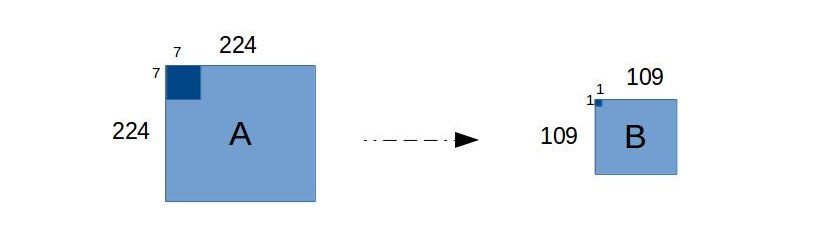
\includegraphics[width=5in]{Figures/conv.jpg}
	\caption[An Electron]{Application d'un filtre de convolution.}
	\label{fig:Electron}
\end{figure}

	La valeur du stride représente le nombre de pixels de déplacement d'un filtre sur une image après chaque opération de convolution. Le passage d'une image à travers une pile de convolution aura pour effet de changer la dimension (nombre de pixels) de l'image. Posons $S$ la valeur du stride, $P$ la valeur du zero-padding, $W_{1}$ le nombre de pixels d'une dimension (longueur ou bien largeur) d'une image et $F$ la taille des filtres de convolution. Pour calculer la taille obtenue en sortie $W_{2}$, on applique la formule suivante:
$$W_{2} = (W_{1} - F + 2*P)/S + 1$$
$$Exemple de la première convolution: (224 - 7 + 2*0)/1 +1 = 109.5$$
	
	Si on obtient un nombre non entier (avec une virgule) comme l'exemple ci-dessus, ce qui représente une opération de convolution incomplète, on prend donc que la partie entière. Comme les images en entrée ont la même largeur et longueur (images carrées), il suffit seulement de calculer cette valeur (nouvelle dimension) pour une seule dimension.
	Cette première couche de convolution est la seule couche sur laquelle on applique une normalisation [Kri et al.,12]. Après cela, on applique un max-pooling sur la sortie résultante des convolutions, comme le montre la figure suivante:

\begin{figure}[H]
	\centering
		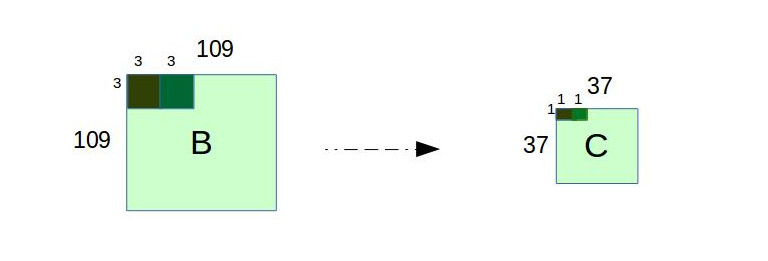
\includegraphics[width=5in]{Figures/pool.jpg}
	\caption[An Electron]{Application d'un max-pooling.}
	\label{fig:Electron}
\end{figure}

	En posant $W_{1}$ le nombre de pixels d'une dimension d'une image, $F$ la taille du max-pooling et $S$ la valeur du stride qui est égale à $F$. On peut calculer la taille du résultat $W_{2}$, comme suit:

$$W_{2} = (W_{1} - F )/S + 1$$
$$Exemple du premier max-pooling: (109 - 3)/3 +1 = 36.33$$

	Ces étapes sont presque les mêmes pour chaque couche de convolution, chacune applique des filtres de convolution d'une certaine taille, suivi ou non d'un max-pooling. On remarque sur la figure qui va suivre dans la troisième couche de convolution, que la taille de l'entrée est de 17x17 et de la sortie 17x17, comme on a dit dans le chapitre précédent cela est dû au zero-padding qui permet de contrôler la dimension des sorties. On remarque aussi que la plus petite taille des filtres de convolution est de 3x3 pixels, et cela pour capturer la notion de gauche / droite, haut / bas, au centre.

	Les sorties obtenues après le passage d'une image sur ces couches de convolutions sont 512 matrices de taille 6x6 pixels, 512 étant le nombre de filtres appliqués lors de la dernière convolution, et la taille 6x6 pixels est la taille de la sortie de cette même couche après application des filtres de convolution et du max-pooling.

	L'empilement des couches de convolution est suivi par trois couches (les 3 dernières couches du tableau) entièrement connectées (Fully-Connected Layers), pour faire passer en entrée les valeurs des sorties des convolutions on devra aplatir les matrices obtenues précédemment (521 matrices de 6x6 pixels) en un vecteur unidimensionnel, comme le montre la figure suivante:

\begin{figure}[H]
	\centering
		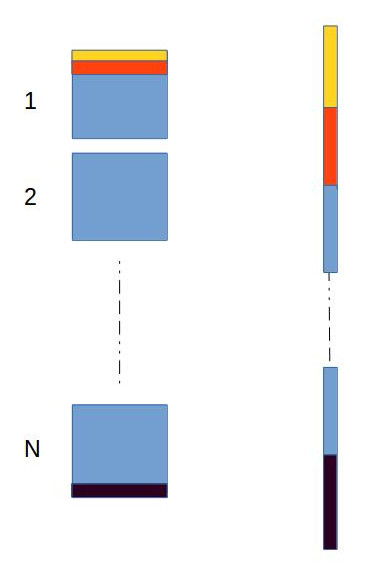
\includegraphics[width=2.5in]{Figures/flattening.jpg}
	\caption[An Electron]{Applatissement des résultats du ConvNets.}
	\label{fig:Electron}
\end{figure}

	Le vecteur unidimensionnel sera composé de la succession des lignes de la première matrice, ensuite les lignes de la deuxième matrice, et ainsi de suite jusqu'à la dernière matrice. Donc dans notre cas, à partir de 512 matrices de 6x6 nous aurons un vecteur unidimensionnel de taille: $512*6*6 = 18432$.

Les deux premières couches entièrement connectées ont 4096 neurones chacune, la troisième et dernière couche du réseau est la couche soft-max. Elle réalise la classification de la base d'image ILSVRC-2012 et contient donc 1000 neurones (un pour chaque classe), cette couche soft-max donnera comme sortie un vecteur de 1000 valeurs contenant les probabilités d'appartenance d'une image aux 1000 classes.

	La figure suivante montre l'architecture complète contenant la taille de chaque entrée et sortie de chaque couche du réseau à convolution:

\begin{figure}[H]
	\centering
		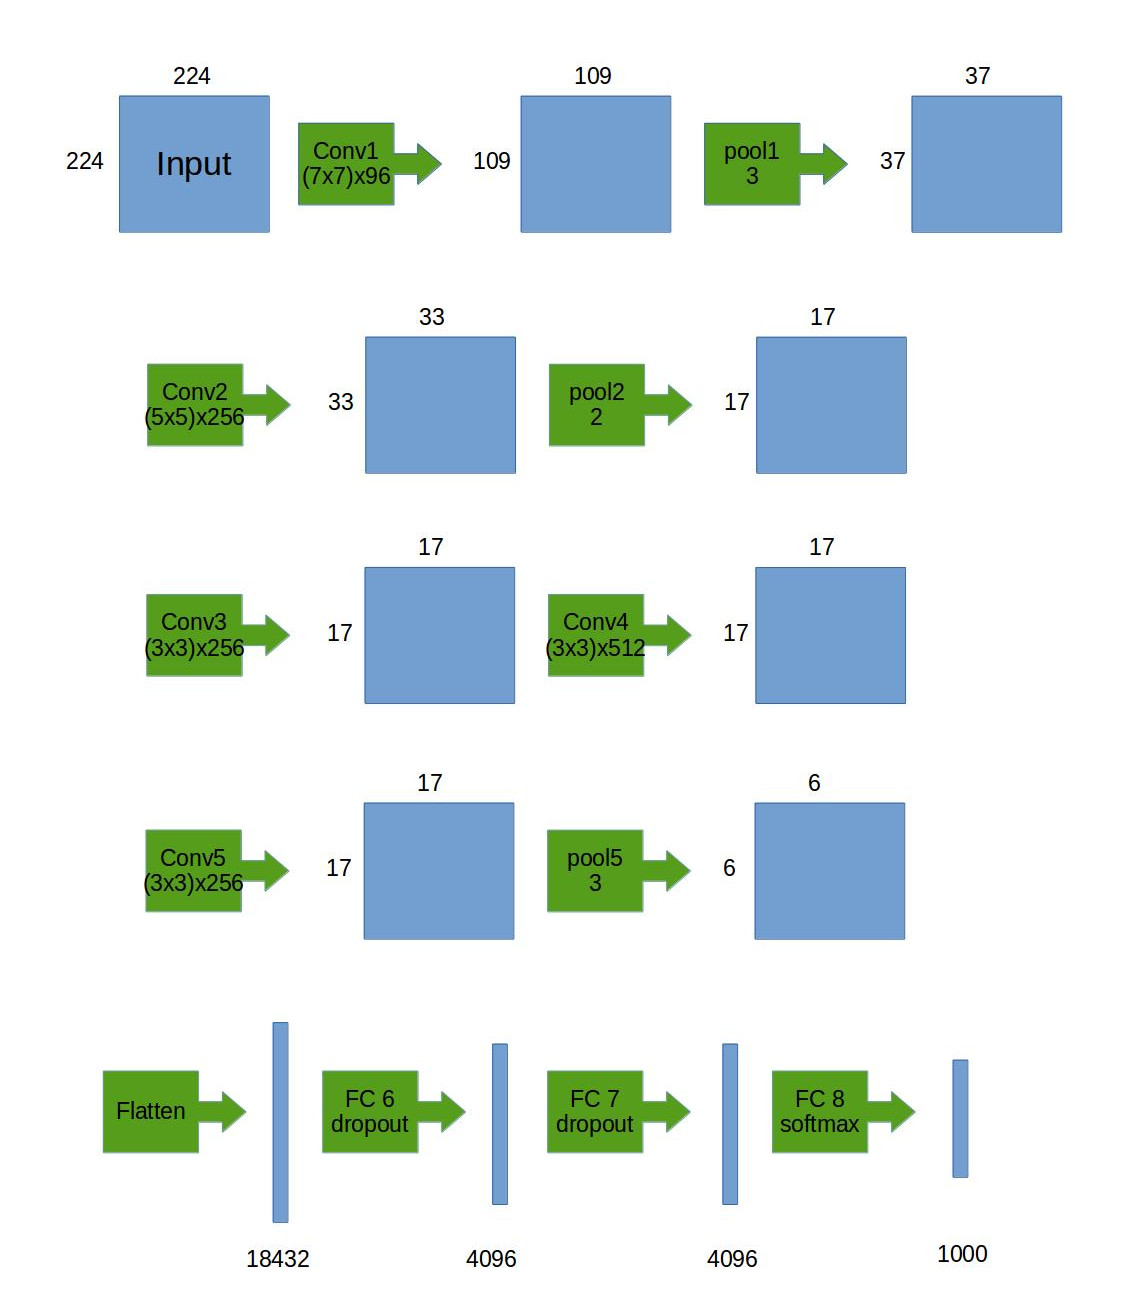
\includegraphics[width=6in]{Figures/architectureVGG.jpg}
	\caption[An Electron]{Architecture complète du ConvNets.}
	\label{fig:Electron}
\end{figure}



\section{Entraînement du réseau}
	Comme pour un réseau de neurones ordinaire, un réseau de neurones à convolution a besoin d'être entraîné sur une base d'exemple (base d'images dans notre cas), plus le réseau a une grande taille (plusieurs poids) plus on aura besoin d'un plus grand nombre d'exemples pour son entraînement. 
	
	La base utilisée pour l’entraînement (apprentissage) de ce réseau à convolution est ILSVRC-2012 (plus de 1.2 million d'images), et l'apprentissage s'est fait avec une descente du gradient stochastique avec moment. Les paramètre empiriques (hyper-paramètres) sont comme suit: Un moment de $0.9$, une dégradation des pondérations (weight decay) $de 5*10^{-4}$, et un taux d'apprentissage initial (learning rate) de $10^{-2}$. [Cha et al.14]
	
	Les valeurs initiales des poids ne peuvent pas être toutes égales à zéro (ou une autre valeur), puisque tous les poids vont calculer le même gradient lors de la rétro-propagation, ce qui résultera en l'application des mêmes mis-à-jours sur tous les poids. En d'autres termes, il n'y aura pas d’asymétrie entre les valeurs des poids si elles sont toutes initialisées à une même valeur. [CS231n 16]	
	Il serait donc plus judicieux d'initialiser les valeurs des poids à des valeurs aléatoires proches de zéro. Pour l'architecture VGG-CNN-S, les valeurs des poids de chaque couches ont été initialisées avec une distribution Gaussienne avec une moyenne de 0 et une variance de $10^{-2}$. [Cha et al.14]
	
	Il est évident que pour réaliser l’entraînement d'un aussi grand réseau requiert de très grands temps de calculs et une très grande puissance CPU/GPU de calculs. L'équipe Visual Geometry Group a utilisé pour cela une carte graphique NVIDIA GTX Titan, l'entraînement du réseau à convolution a duré pendant 3 semaines, sans inclure le temps de paramétrage des hyper-paramètres (moment, learning rate, etc.).
	
	Comme dans notre cas, nous ne disposons pas d'une aussi grande puissance de calcul ni le temps nécessaire pour paramétrer le réseau à convolution, nous ne pouvons pas réaliser l’entraînement de ce réseau. L'équipe VGG a eu donc la courtoisie de publier pour les chercheurs les poids que leurs réseaux (VGG-CNN-S et autres) ont appris durant la phase entraînement, nous n'avons donc pas eu à refaire ce qui a été fait.


\section{Extraction des caractéristiques}
	L'architecture du réseau à convolution utilisée contient une succession de piles de convolutions qui se termine par des couches entièrement connectées, nous allons nous intéresser à ses dernières dans nos approches de comparaisons pour notre algorithme de recherche d'image par le contenu.
	Pour cela nous allons prendre chaque image et l'envoyer en entrée du réseau à convolution, et comme nous avons les différents poids de l'architecture VGG-CNN-S, nous pourrons ainsi récupérer les différentes valeurs que prends une image dans chaque couche du réseau à convolution. Comme les dernières couches du ConvNets sont des couches entièrement connectées, et donc seront sous le format d'une liste de valeurs réelles, nous pourrons manipuler les valeurs obtenues dans ces dernières couches. Le but étant de comparer une même couche de deux images différentes, la comparaison (calcul de ressemblance) se fait en calculant la distance (distance euclidienne) entre ces deux listes de nombre réel.
	
	Nous allons maintenant présenter nos résultats obtenus (mesures de performance) de notre algorithme de recherche d'image par le contenu décrit au début de ce chapitre, en utilisant les trois dernières couches de l'architecture du réseau à convolution (les couches entièrement connectées) comme méthode de comparaison des images. Rappelons aussi que les bases utilisée dans notre algorithme sont les bases WANG et Caltech-101, nos premières approches sont donc comme suit:

\subsection{Dernière couche Soft-max 1000}
	Pour notre première approche, nous avons utilisé pour comparer les images la dernière couche du réseau à convolution qui est la couche Soft-max, cette couche contient 1000 valeurs (une valeur pour chaque classe de ILSVRC-2012) rappelons que cette couche contient les probabilités d'appartenance d'une image aux 1000 classes. Nos résultats obtenus sont comme suit:	

\begin{figure}[H]
\begin{center}
\begin{tabular}{|c|c|c|c|c|c|c|c|}
\hline
	Mesure & 1-Préc & 5-Préc & 10-Préc & 20-Préc & 40-Préc & 60-Préc & Rappel\\
\hline
	WANG & 0.86 & 0.846 & 0.804 & 0.715 & 0.606 & 0.531 & 0.442\\
\hline
	Caltech-101 & 0.551 & 0.512 & 0.479 & 0.431 & - & - & 0.321\\
\hline
\end{tabular}
\end{center}
\caption{Résultats obtenus avec la dernière couche de 1000 valeurs.}
\end{figure}

	Nous remarquons que pour la base WANG nous avons un très bon taux de 1-Précision de 86\% soit un taux d'erreur de 14\% seulement. En d'autres termes notre algorithme de recherche d'image avec cette approche arrive à trouver dans 86\% des cas que l'image la plus ressemblante à une image requête appartient à la même classe que la requête. Quand à la base Caltech-101 nous avons un taux de 55.1\% de 1-Précision, rappelons que cette base contient beaucoup plus d'images et surtout plus de classes par rapport à la base WANG, ce qui diminuera la probabilité que l'algorithme arrive à trouver que l'image la plus ressemblante appartient à la même classe que l'image requête.
	Globalement nous remarquons aussi que plus nous demandons un nombre plus grand d'images ressemblantes à une requête: top-1 avec la 1-Précision, top-5 avec la 5-Précision et ainsi de suite jusqu'au Rappel qui essaye de trouver exactement le nombre total d'images de la même classe, et plus notre algorithme a du mal à les trouver.
	Ces résultats sont acceptables, sachant que les classes des base WANG (10 classes) et Caltech-101 (101 classes) ne sont pas incluent dans les 1000 classes de la base ILSVRC-2012 d’entraînement du réseau. Donc ce sera plus difficile à la couche Soft-max de trouver une approximation des classe des deux bases en utilisant les 1000 probabilité d'appartenances de ILSVRC-2012.
	On peut donc dire qu'avec cette couche, nous effectuons une recherche par étiquette (label) de classes de ILSVRC-2012. 

%Dans cette approche nous avons utilisé les valeurs de la dernière couche du ConvNets pour la comparaison (calcul des distances). Cette couche contient 1000 valeurs chacune représentant la probabilité d'appartenance de l'image à l'une des 1000-ILSVRC classes de la base utilisée dans l'entraînement [Rus et al.15].
%SUPPOSITION : Résultats acceptables mais non satisfaisants.




\subsection{Avant avant dernière couche de 4096 valeurs} 
	Dans cette deuxième approche nous intéresserons à l'avant avant dernière couche du réseau à convolution, c'est la première couche entièrement connecté qui se trouvent après les piles de convolution. Cette couche contient 4096 valeur, par conséquent on la notera comme la couche \textbf{4096a}. Contrairement à l'approche précédente, cette couche n'est pas une soft-max donc elle ne contient pas la classification de la base ILSVRC-2012 en 4096 classes. Mais plutôt elle contient une représentation de l’aplatissement des 512 matrices 6x6 obtenues à partir des piles de convolutions (cumul des apprentissages des convolutions), et elle a été transformée en 4096 valeurs dans cette couche. En utilisant les 4096 valeurs de cette couche pour le calcul des ressemblance, nous avons obtenu les résultats suivants:

\begin{figure}[H]
\begin{center}
\begin{tabular}{|c|c|c|c|c|c|c|c|}
\hline
	Mesure & 1-Préc & 5-Préc & 10-Préc & 20-Préc & 40-Préc & 60-Préc & Rappel\\
\hline
	WANG & 0.840 & 0.796 & 0.762 & 0.715 & 0.653 & 0.583 & 0.514\\
\hline
	Caltech-101 & 0.654 & 0.521 & 0.454 & 0.371 & - & - & 0.257\\
\hline
\end{tabular}
\end{center}
\caption{Résultats obtenus avec la couche 4096a.}
\end{figure}

	Nous remarquons que ces résultats sont assez différents de ceux obtenus avec la couche soft-max de 1000. Pour la base WANG: la 1-Précision, 5-Précision et 10-Précision ont diminué de 2\% à 5\%, mais à partir de 20-Précision jusqu'au Rappel nous avons une augmentation de reconnaissance, donc l'algorithme a plus de difficulté à trouver les images les plus ressemblantes, mais arrive à trouver mieux toutes les images ressemblante de la même classe.
	Quant à la base Caltech-101: c'est le contraire, il arrive mieux à retrouver les images les plus ressemblantes mais moins toutes les images ressemblantes de la même classe.
	En résumé la couche 4096a ne donne pas forcément de meilleurs résultats que la couche soft-max 1000. Cela dépend du nombre de classes et d'exemples de chaque base d'images. On peut dire que contrairement à la recherche par étiquette effectuée dans la couche Soft-max 1000, nous effectuons avec la 4096a ce que nous appelons comme recherche sémantique. Sémantique parce-que elle compare les images grâce aux informations cumulées à partir des piles de convolutions.

%C'est la première couche de neurones entièrement connectés (4096 neurones), celle qui se trouvent juste après les couches de convolution. Cette couche cumule donc l'apprentissage des dernières convolutions qui ont été effectué sur l'image.
%SUPPOSITION: Cumuler les informations sémantiques qui sont traitées moins profondément.

\subsection{Avant dernière couche de 4096 valeurs}
	La couche qui sera utilisée pour notre troisième approche est l'avant dernière couche entièrement connectée du réseau à convolution. Elle contient 4096 valeurs et se trouvent entre la couche Soft-max 1000 et la couche 4096a, on la notera donc comme la couche \textbf{4096b}.
	La couche 4096b ajoute un traitement plus avancé des connaissances acquises à partir de la couche 4096a qui la précède, et n'étant pas une Soft-max donc elle ne donne pas une représentation en classes, elle est par conséquent moins spécialisé que la dernière couche Soft-max 1000.


\begin{figure}[H]
\begin{center}
\begin{tabular}{|c|c|c|c|c|c|c|c|}
\hline
	Mesure & 1-Préc & 5-Préc & 10-Préc & 20-Préc & 40-Préc & 60-Préc & Rappel\\
\hline
	WANG & 0.97 & 0.947 & 0.932 & 0.900 & 0.855 & 0.795 & 0.716\\
\hline
	Caltech-101 & 0.773 & 0.681 & 0.627 & 0.540 & - & - & 0.405\\
\hline
\end{tabular}
\end{center}
\caption{Résultats obtenus avec la couche 4096b.}
\end{figure}

	Les résultats des mesures de performances en utilisant cette couche pour la comparaison sont nettement meilleurs qu'en utilisant les couches des deux approches précédentes, pour les deux bases WANG et Caltech-101 nous avons une très grande amélioration dans chacune des N-Précisions ainsi que le Rappel. Ces amélioration varient de 10\% jusqu'à plus de 20\% d'augmentation.
	Pour la base WANG nous avons une 1-Précision de 97\%, l'algorithme avec à trouver presque dans tous les cas la bonne image la plus ressemblante. Quand aux résultats de la base Caltech-101, ils ne sont pas aussi bons que ceux de WANG mais nous obtenons de très bonnes améliorations sur toutes les mesures de performance. 
	Nous remarquons donc que la couche 4096b est la meilleure couche pour comparer les images avec notre algorithme, mais nous pouvons dire aussi que c'est la meilleure couche qui permet de donner la meilleure description d'une image donnée, une description sémantique qui ne dépend pas de la classe de l'image mais de l'information sémantique de son contenu. Avec cette couche nous arrivons à mieux rassembler les informations sémantiques obtenus des convolutions et de la couche 4096a sans être spécialisée en classes comme la couche Soft-max 1000.

%Cette l'avant dernière couche du ConvNets, elle se trouve donc entre les deux couches précédemment utilisées. C'est une couche entièrement connectée qui contient 4096 neurones.
%Cette couche ajoute un traitement plus avancé des connaissances acquises de la couche qui la précède (4096a) mais elle est moins spécialisé que la dernière couche (1000 neurones par classes)
%SUPPOSITION: Rassembler les informations sémantiques obtenus des convolutions et de la couche précédente sans être classifiées en 1000 classes.


%\section{Sur quoi se base notre approche ?}
\section{La description sémantique}

Pour expliquer les résultats, nous devons comprendre ce qui se passe dans le réseau à convolution. Jusqu’à dernièrement, il n'y avait pas beaucoup de preuve sur ce qui se passait durant l'apprentissage, ce qui n’était pas satisfaisant d'un point de vue scientifique.


L'approche de [Zei et al. 14] nous a permis de trouver une théorie bien fondée pour expliquer l'apprentissage qu'effectuent les ConvNets. Il montre dans sa recherche comment les différents masques de convolutions finissent par se spécialiser en apprenant à reconnaître un motif précis. Les filtres de couches profondes apprennent à reconnaître des motifs plus complexes en combinant les résultats des convolutions des couches précédentes.
Ainsi, on trouve que le réseau imite finalement bien le comportement hiérarchique observé dans le cerveau.


L’étude observe aussi l’évolution des caractéristiques apprisent par les masques de convolution avec l’entraînement et fait une analyse de sensibilité (sensitivity analysis) qui consiste à tester le comportement du réseau et les résultats de détection quand on cache certaines partie de l'image.

\begin{figure}[H]
	\centering
		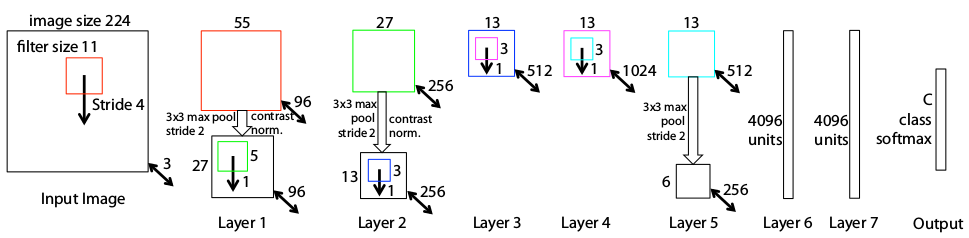
\includegraphics[width=5in]{Figures/arch.png}
	\caption[Res]{Architecture utilise pour le conv net.}
	\label{fig:Electron}
\end{figure}


Le travail s'est basé sur [LeCun et al. 89] et [Kri et al. 12] qu'il a entraîné sur la base d'image de ImageNet 2012 qui contient 1,3 million d'image RGB et 1000 classes. L'Entropie croisée (cross-entropy) fut utilise pour le calcule d'erreur. L’entraînement a été effectué par descente du gradient avec des mini-batch d'une taille de 128 images, un taux d'apprentissage de 0.01 et un dropout sur les dernières couches d'une valeur de 0,5 . Les poids furent initialise à 0.01 et les biais à 0.


[Zei et al. 14] propose dans leur travail une nouvelle manière de retracer les activités des masques de convolution et des caractéristiques qu'ils apprennent vers les pixels qui les ont excite a l'aide de réseaux de déconvolution. Ces derniers reprennent la même architecture que les réseaux a convolution, mais d'une manière inverse. Ils effectuent dans l'ordre suivant: \textbf{Unpooling}: le max-pooling généralement utilise n'est pas inversible. Pour approximer l'inverse de ce dernier l’Idée est donc de sauvegarder l'emplacement du maximum pour chaque région de pooling. Voir figure[]. \textbf{Rectification}: qui s'effectuent a travers l'application de la non linéarité "relu" qui ne fait que prendre le maximum entre la valeur en entrée et 0 pour garder les résultats positifs. Enfin, le \textbf{Filtering}: la dernière étape est d'appliquer les inverses des filtres de convolutions . Ces derniers sont considéré comme étant les transpose des filtres appris. La transpose étant calcule par inversant chaque filtre horizontalement et verticalement.


\begin{figure}[H]
	\centering
		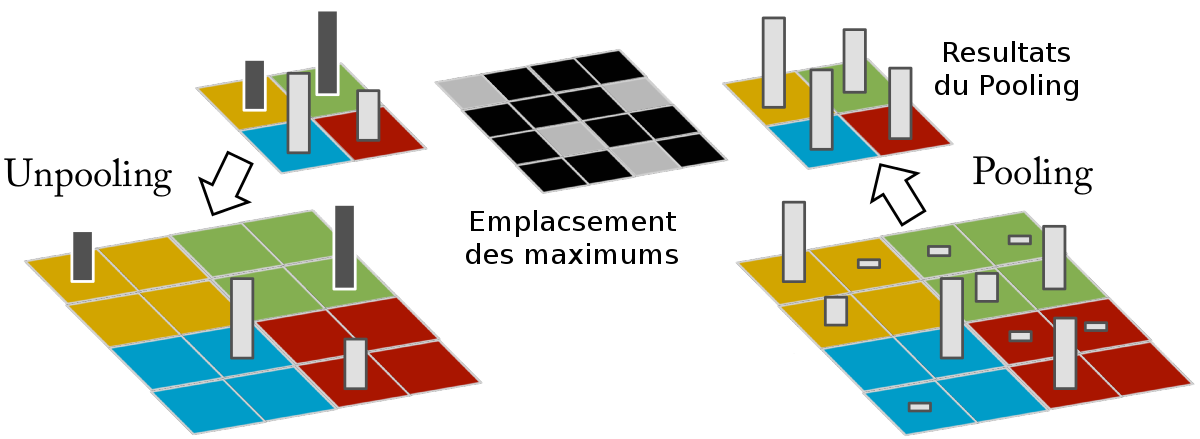
\includegraphics[width=5in]{Figures/unpooling.png}
	\caption[Res]{Chema descriptif du Unpooling.}
	\label{fig:Electron}
\end{figure}

\textbf{Visualisation des caractéristiques}

La tache de visualisation tente de donner un sens a l'apprentissage. Montrer ce que chaque masque détecte peut nous éclaircir sur le sujet. L'approche est donc de tenter de trouver  les zones d'images en entrée qui sont a l'origine de l'activation de chaque masque. 

Par soucis de temps, nous n'avons pas pu implémenter les déconvolutions sur nos modèles. Les résultats obtenu par [Zei et al. 14] sont représenté sur la figure, elle représente le top 9 des zones qui causent le plus grand taux d'activation pour un masque donnée.

On peut voir la nature hiérarchique de la reconnaissance, dans les premières couches, des formes basique sont détecté (la détection de différentes lignes par la couche 1, différents types de coins par la couche 2) et combine d'une couche a une autre pour arriver a des représentations plus complexe (des textures dans la couche 3), jusqu’à pouvoir reconnaître des objets plus significatif dans les dernières couches (humain, chien, roue, fleure ...etc). 

\begin{figure}[H]
	\centering
		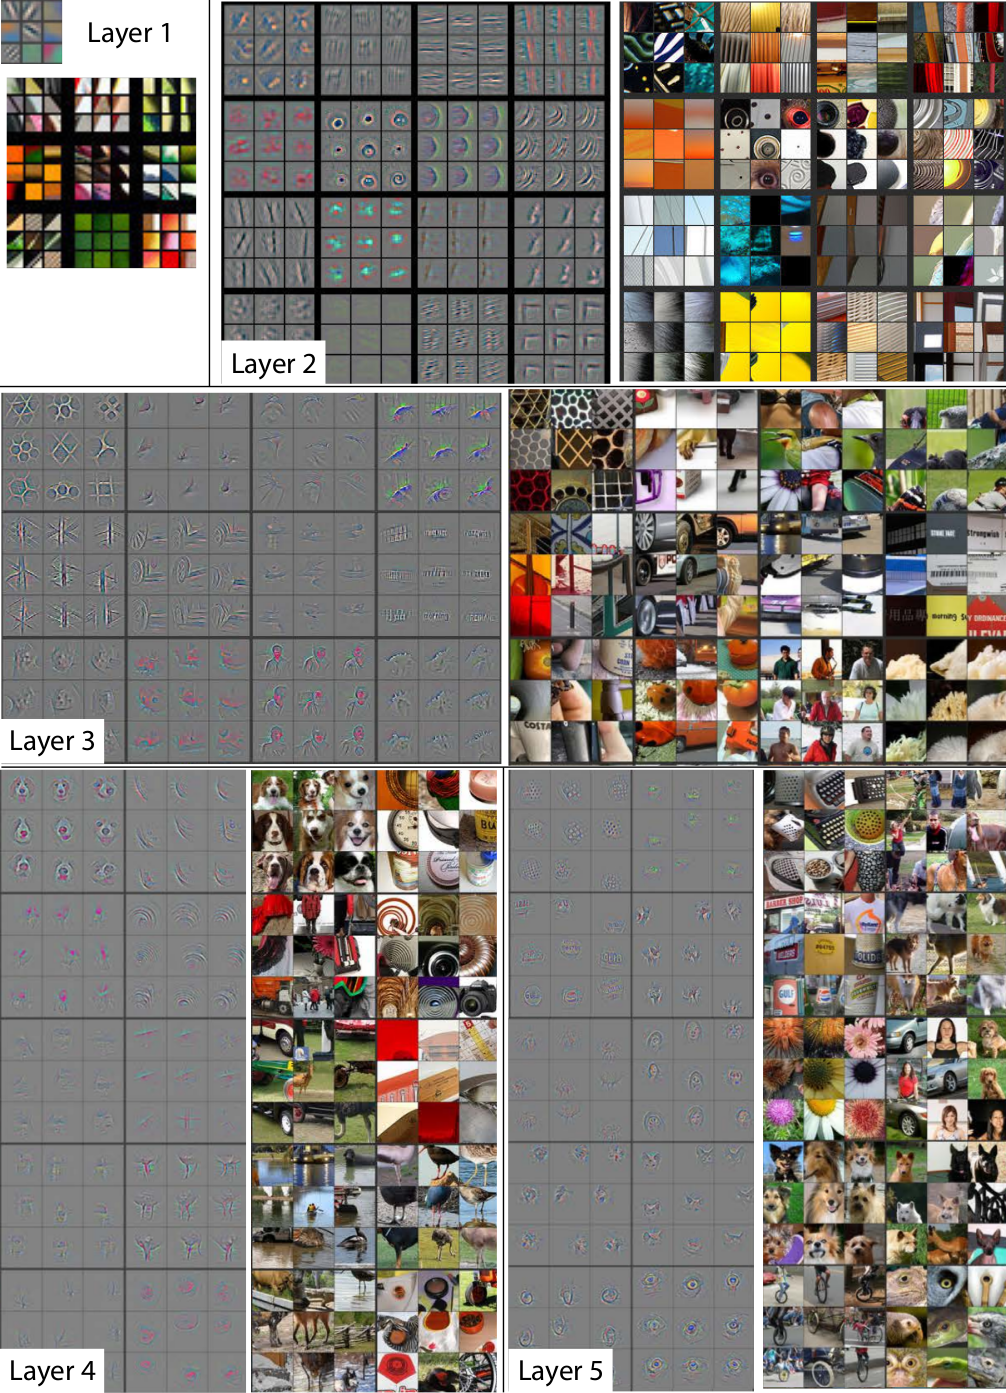
\includegraphics[width=5in]{Figures/visualisation.png}
	\caption[Res]{Visualisation des differentes de l'apprentissage des differentes couches.}
	\label{fig:Electron}
\end{figure}

Mais la aussi, nous savons pas a coup sure si la détection se fait par rapport aux objets, ou a ce qu'ils ont au tour. Pour remédier a ce problème, certaine partie de l'image ont été cachées (avec des rectangles gris), les résultats des testes montrent que le taux de reconnaissance diminue d'une façon radicale, ce qui prouve donc que la détection se fait bien sur les objets eux mêmes.

Nous pouvons donc assumer qu'au final, la représentation retournée par le réseau est bien une représentation sémantique du contenue de l'image qui décris d'une certaine façon son contenue. C'est cette représentation qui sera traduite en termes (1000 libelle des classes) a travers la dernière couche de softmax. Cette représentation force le réseau a utiliser des termes bien précis pour exprimer ce qu'il a appris. C'est de cette raison qu'on retrouve donc de meilleur résultats lors de l'utilisation des sorties de l'avant dernière couche (4000b) ou les concepts appris sont encore libre de cette contrainte. Enfin, plus les représentations sont traites en profondeur, plus elles sont significatifs, et plus le réseau apprend des concepts plus complexes. C'est par ceci que sont expliqués les résultats pas très bons de l'avant avant dernière couche (4000a) (on remarque que les résultats de la couche de softmax (1000) se rapproches de celle de (4000a)).

\subsection{Autoencoder 4x1x4 A REFAIRE} Application d'un réseau d'autoencoder sur les valeurs de la couche 4096b, ce sera un apprentissage qui aura pour but de codifier (convertir) les 4096 valeurs en seulement 1000 valeurs. Ce réseau à une architecture très simple qui est comme suit: 4096 neurones dans la couche d'entrée, 1000 neurones dans la couche cachée et 4096 neurones dans la couche de sortie.
SUPPOSITION: Obtenir de meilleurs résultats que la première approche qui utilise la dernière couche de 1000 neurones par classe.

\begin{figure}[H]
	\centering
		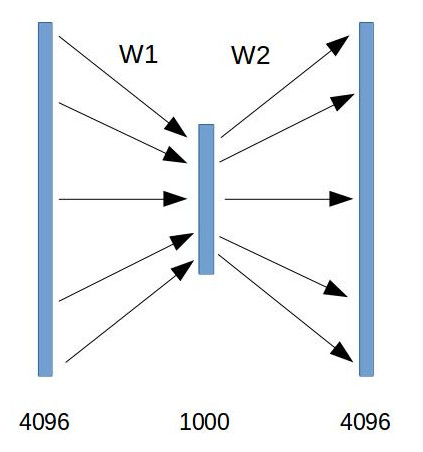
\includegraphics[width=2.5in]{Figures/ae/414.jpg}
	\caption[An Electron]{Architecture Autoencoder 4x1x4.}
	\label{fig:Electron}
\end{figure}

\subsection{Autoencoder 4x2x1x2x4 A REFAIRE} Cette approche utilise une autre architecture d'un réseau autoencoder qui est plus profond que le précédent. Son architecture est comme suit : Une couche d'entrée de 4096 neurones, trois couches cachées ayant dans l'ordre 2000, 1000 et 2000 neurones et finalement la couche de sortie de 4096 neurones.
SUPPOSITION: Obtenir un meilleur taux d'apprentissage que l'autoencoder précedent.

\begin{figure}[H]
	\centering
		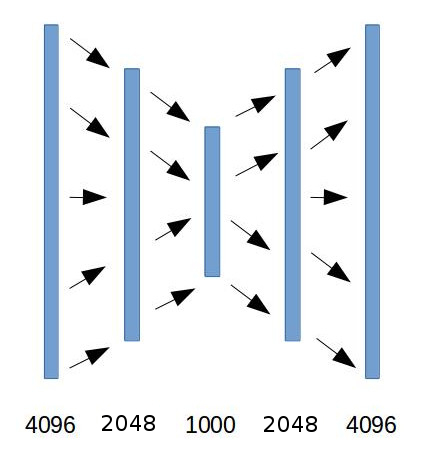
\includegraphics[width=2.5in]{Figures/ae/42124.jpg}
	\caption[An Electron]{Architecture Autoencoder 4x1x4.}
	\label{fig:Electron}
\end{figure}


\subsection{Denoising autoencoder 4x1x4 A REFAIRE} Nous avons tester un autoencoder plus complexe. C'est la même architecture que l'autoencoder 4x1x4, mais avec un taux de corruption de 30\% et moins de paramètre pour éviter au maximum le sur-apprentissage.
SUPPOSITION: Forcer un apprentissage plus significatif et réaliste.

\begin{figure}[H]
	\centering
		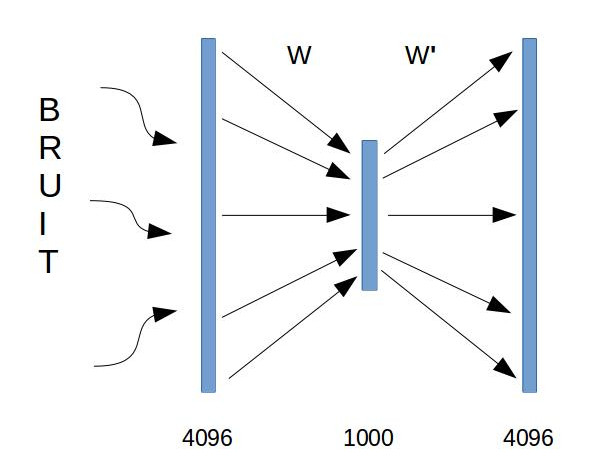
\includegraphics[width=3in]{Figures/ae/denoising.jpg}
	\caption[An Electron]{Architecture Autoencoder 4x1x4.}
	\label{fig:Electron}
\end{figure}

\subsection{Autoencoder 4x1x4 A REFAIRE} avec descripteurs (SIFT,LBP,GLCM,formes,couleurs) : L'architecture de ce réseau ressemble un peu aux précédentes, sauf qu'au lieu de donner en entrée/sortie seulement les 4096 valeurs, on va leurs rajouter différents descripteurs. La combinaison de ses valeurs devra être codifié en 1000 valeurs dans la couche cachée.
 
SUPPOSITION: On ne sait pas si les descripteurs "fabriqués à la main" vont aider à améliorer l'apprentissage ou bien non. Le cerveau n'effectue pas ce genre de calcul, mais l'architecture de l'ordinateur peut lui permettre d'exploiter ses différents descripteurs pour une meilleure reconnaissance.


\begin{figure}[H]
	\centering
		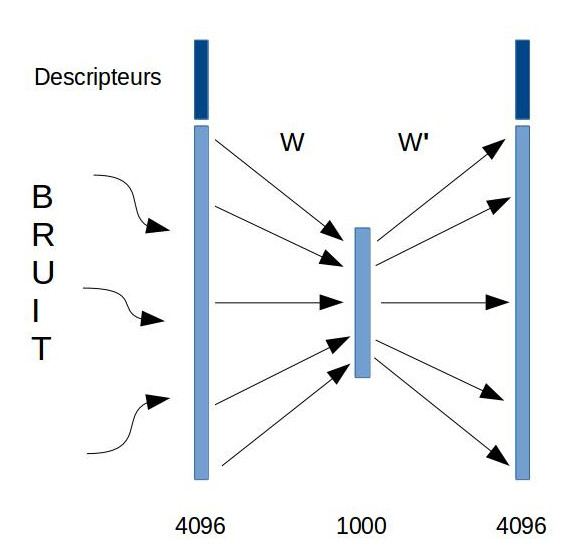
\includegraphics[width=3in]{Figures/ae/AE-Descripteur.jpg}
	\caption[An Electron]{Architecture Autoencoder 4x1x4.}
	\label{fig:Electron}
\end{figure}



\section{EXPLICATION AUTOENCODERS:}
En plus de réduire l'espace de représentation pour prouver que c'est finalement pas ce dernier qui influe sur les résultats, l'utilisation d'auto-encoder ont montré une amelioration considérable des résultats de recherches d'images.

Pour comprendre pourquoi ceci s'est produit nous explorons plus en détails le fonctionnement de l'autoencoder (AE) [Ian et al 2016]. L’idée est, comme expliqué précédemment, dans le chapitre 2, que les données sont concentrées autour d'une partie d'un espace d'une dimension inférieure (appelée Variété ou Manifold) a celle de l'espace de représentation actuelle des données. L'objectif est de retrouver la structure de ce premier. L'AE effectue ceci en faisant le compromis entre deux contraintes (i) Apprendre une représentation \textbf{h} d'un exemple en entrée \textbf{x} (\textbf{h} etant généralement d'une dimensionnalité plus faible) tel que \textbf{x} peut être récupéré a partir de \textbf{h} grâce a un décoder et ce avec un minimum d'erreur. Si \textbf{x} n'appartient pas à l'espace de données en entrée, la reconstruction n'est pas sensée donner de bon résultats. (ii) Le deuxième points à satisfaire est l'ensemble de contraintes de régularisation qui est infligé à l'autoencoder qui ont généralement pour but d’éviter le sur-apprentissage et permettre donc d'avoir une représentation plus générale.


\begin{figure}[H]
	\centering
		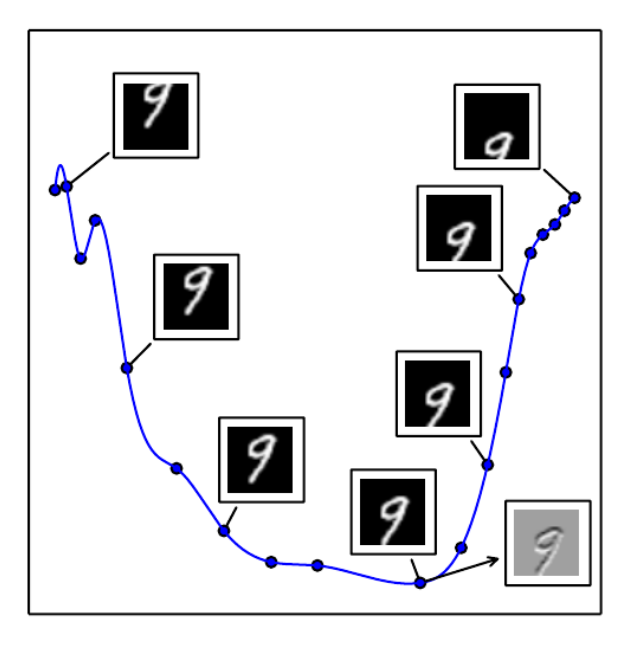
\includegraphics[width=3.5in]{Figures/manifold.png}
	\caption[Res]{Exemple d'une Variété à une dimension dans un espace de 784 dimensions des images de la base MNIST (28×28 pixels). Une image fut prise et déplacée verticalement. Le taux de déplacement vertical défini des coordonnes qui retrace une courbe. Pour la visualiser, cette dernière a été projeté vers un espace 2 dimensions en utilisant PCA (Principal Component Analysis). }
	\label{fig:Electron}
\end{figure}


Nous expliquons donc, dans notre cas, la hausse de niveau de precision par le fait que les représentations sémantiques retenus par le réseau a convolution soient compressé par le "coder", il constitue dorénavant un moyen de résumer les représentations en les combinant d'une façon à en garder ce qu'il y a de plus essentiel.

Ensuite, les contraintes ajouté au Denoising AE lui ont permise d'apprendre une compression plus générale, d’où ses résultats remarquables.

Comparer ces représentations compressées donne donc de meilleurs résultats pour la recherche d'image par contenue.


\section{Conclusion}

Nous concluons ce chapitre en constatant que les méthodes d'apprentissage profond donnent effectivement des résultats très satisfaisants quand on les appliques au problème de recherche d'image par contenue. Même si nos approches pourraient être développé pour donner de meilleur résultats, et en performance, et en temps d’exécution. Nous allons, dans le prochain chapitre, aborder certain détails techniques, mais aussi visualiser concrètement certain résultats de différentes images en requêtes.